%File: submission_v4.tex --- AAAI-27 anonymous submission (C14-integrated revision)
% "An Empirical Analysis of Transfer for Dynamic Path Planning"
% Built on the official AAAI-27 author kit (aaai2027.sty, TemplateVersion 2027.1).
\documentclass[letterpaper]{article} % DO NOT CHANGE THIS
\usepackage[submission]{aaai2027}  % DO NOT CHANGE THIS
\usepackage[hyphens]{url}  % DO NOT CHANGE THIS
\usepackage{graphicx} % DO NOT CHANGE THIS
\urlstyle{rm} % DO NOT CHANGE THIS
\def\UrlFont{\rm}  % DO NOT CHANGE THIS
\usepackage{natbib}  % DO NOT CHANGE THIS AND DO NOT ADD ANY OPTIONS TO IT
\usepackage{caption} % DO NOT CHANGE THIS AND DO NOT ADD ANY OPTIONS TO IT
\frenchspacing  % DO NOT CHANGE THIS
%
% Recommended for better-looking tables
\usepackage{booktabs}
\usepackage{amsmath}
%
\pdfinfo{
/TemplateVersion (2027.1)
}
\setcounter{secnumdepth}{0}

% Custom macros

\title{An Empirical Analysis of Transfer for Dynamic Path Planning}
\author{
    Anonymous Submission
}
\affiliations{
}

\begin{document}

\maketitle

\begin{abstract}
We study the dynamic path planning problem, where an agent needs to plan a route in the presence of moving obstacles. This problem is relevant for all agents that need to navigate in the real world. In particular, we study whether heuristics learned in training maps can be transferred---zero-shot or from a few labeled target maps---to new environments for this task. We show that, with the right training objective and planner integration, heuristics transfer zero-shot in both discrete and continuous environments---even heuristics given no information about future obstacle motion---matching or improving success in new maps while substantially reducing search effort. With a few labeled target maps, low-rank adaptation preserves the transferred prior while full fine-tuning overtakes it as labels accumulate---and a matched-label factorial shows that the diversity of target worlds, not raw label count, governs when full fine-tuning is safe. Further, across comparable backbones no architecture is uniformly best: Multilayer Perceptrons, Long Short-Term Memory models, Hierarchical Reasoning Models and U-Net architectures can all support this transfer, while hierarchy-specific gains do not persist across the tested formulations.
\end{abstract}

% Uncomment the following to link to an anonymous code/data archive included with the submission.
% Keep this block between (not within) the abstract and the main body.
% \begin{links}
%     \link{Code and Data}{https://anonymous.example/}
% \end{links}

\section{Introduction}

Dynamic path planning searches over both configuration and time: when obstacles move, a planner must consider waiting, detouring, and timing, and the search space grows accordingly \citep{silver2005cooperative,phillips2011sipp}. The geometric admissible heuristics that make A\textsuperscript{*} \citep{hart1968astar} efficient on static maps ignore exactly these temporal effects, so search effort grows sharply in the presence of moving obstacles. Learned heuristics can reduce search effort \citep{arfaee2011bootstrap,bhardwaj2017sail,yonetani2021neuralastar}, but a deployed planner benefits only if a heuristic trained on one set of maps remains useful on maps it has never seen. We study zero-shot and few-shot transfer of learned heuristics to unseen environments for dynamic path planning.

We organize the experiments around three factors---the training formulation, the way the prediction enters the planner, and the distribution of target supervision---and isolate each with matched controls where the design permits. Each factor is first evaluated on static suites, where supervision is exact and confounds are controllable, and the resulting choices are then tested under deterministic dynamics. Comparisons use matched controls throughout: twin models differing in one input, identical trained weights under different planner integrations, per-suite expansion budgets calibrated on the classical baseline, and map-level paired inference for repeated evaluations \citep{henderson2018matters,agarwal2021precipice,pineau2021reproducibility}. For the confirmatory experiments, the comparison, evaluation unit, and decision criteria were specified before test evaluation. Across the tested settings, representation, planner integration, and supervision regime explain the observed transfer outcomes more consistently than model family.

Our contributions are:
\begin{itemize}
    \item \textbf{Dynamic zero-shot transfer with one fixed learned heuristic.} A single trained U-Net heuristic---selected on a development cohort, frozen before the confirmation cohort was generated, and given no future-motion input---improves success on all six dynamic test suites of a 50-map-per-suite confirmation cohort ($+0.18$ to $+0.84$; every paired map-level CI excludes zero) and reduces matched search effort on jointly solved maps by 73--95\%. Three of the six suites use map generators never seen in training (family-level transfer); the other three use training families with disjoint maps. Two independently trained models reproduce the success result on the same confirmation cohort.
    \item \textbf{Planner integration changes whether transferred predictions reduce search.} Changing the input--target--output formulation rescues a collapsed recurrent model; changing only the planner integration turns an inert discrete residual into useful guidance; and sharing one search state turns an exact oracle from a six-map loss into a six-map win. A model cannot be blamed for a negative planning result unless its supervised target and search interface are controlled.
    \item \textbf{Target-world diversity governs adaptation stability.} With scarce static supervision, low-rank adaptation preserves the transferred prior while full fine-tuning is unstable; with more supervision, full fine-tuning often overtakes it (direct map-paired contrasts in all six target/backbone cells at both ends). A matched-label factorial attributes the low-supervision failure to concentration of supervision in too few worlds rather than to raw label count: distributing the same labels across more worlds rescues full fine-tuning, while low-rank adaptation never collapses in any tested cell.
\end{itemize}
Additional experiments test the scope of these conclusions: an eight-step future-obstacle window provides no consistent benefit under the tested deterministic dynamics, and descriptor-weighted adapter interpolation and hierarchy-specific depth add no consistent value under the tested formulations. In a restricted-observation study, a locally observed heuristic combined with one Bellman backup reduces expansions against a complete-map comparator under the tested static protocol.

Figure~\ref{fig:dynamic} reports the primary dynamic evaluation. Full protocols, per-suite tables, and statistical details appear in the technical appendix.

\begin{figure*}[t]
\centering
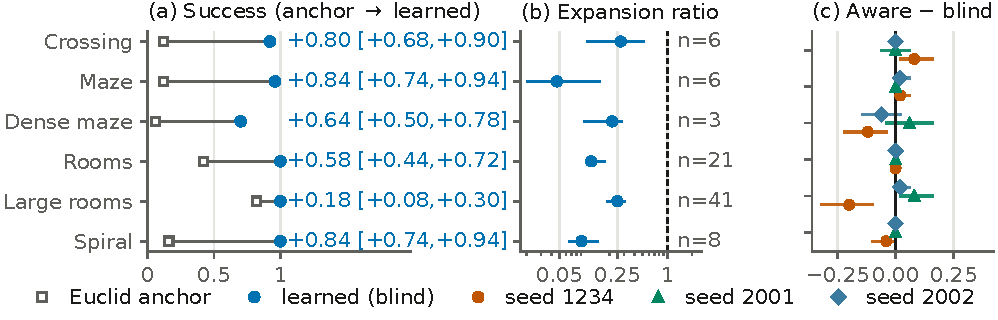
\includegraphics[width=0.98\textwidth]{figures/fig_dynamic_headline.pdf}
\caption{Dynamic zero-shot transfer of one fixed blind U-Net heuristic on the 50-map-per-suite confirmation cohort (dense maze, crossing, and large rooms are family-level held out). (a) Anchor (open squares) and learned (filled circles) success per suite; labels give the paired mean delta with its map-level 95\% CI (all six exclude zero; marginal intervals). (b) Matched-solved expansion ratios on a log axis with map-level 95\% CIs; $n$ is the jointly solved count (dense maze, $n{=}3$, is descriptive). (c) Map-paired aware$-$blind success differences for all three training seeds; the large-rooms cell flips sign across seeds. Per-seed tables and the cohort-disjointness check are in the appendix.}
\label{fig:dynamic}
\end{figure*}

\section{Problem Formulation and Learned-Heuristic Interfaces}

\textbf{Planning problems.} In the continuous setting, a point robot plans on a probabilistic roadmap \citep[PRM;][]{kavraki1996prm} built over a square world of side length $L{=}1.0$ ($2.0$ for the large-room family); units are abstract. Each roadmap contains exactly 192 sampled nodes with $k{=}7$ nearest-neighbor connectivity; the start and goal are inserted as nodes 0 and 1, edges are validated by sampled collision checks at resolution $0.01L$, and worlds whose roadmap does not connect start to goal are rejected. Static search states are roadmap nodes, edge costs are Euclidean lengths $\ell(e)$, and the anchor heuristic is Euclidean distance to the goal, $h_0(v) = \lVert x_v - x_g \rVert$. In the dynamic setting, obstacles move on deterministic trajectories and the search state is a pair $(v,t)$ of node and discrete time step of duration $\Delta t$. The planner may traverse an edge, taking $\tau(e) = \lceil \ell(e) / (v_{\mathrm{agent}} \Delta t) \rceil$ steps, or wait one step; transitions are validated against the obstacle trajectories by sampled collision checks along the edge and interval. Cost is arrival time in steps, search runs to a horizon $t_{\max}$, and the anchor is the travel-time lower bound $h_0(v,t) = \lVert x_v - x_g \rVert / (v_{\mathrm{agent}} \Delta t)$, constant in $t$, so anchor and cost share units. In the discrete setting, agents plan on occupancy grids of $20{\times}20$ to $256{\times}256$ cells with Manhattan distance as the anchor.

\textbf{Supervision targets.} With $h^{*}$ the exact cost-to-go (graph Dijkstra on the static roadmap; backward space--time Dijkstra over $(v,t)$ in the dynamic setting), the regression target is the normalized anchor residual $\bar\delta^{*}(s) = \mathrm{clip}\!\left(h^{*}(s) - h_0(s),\, 0,\, c\,T\right)/T$, where $T$ is the normalization scale ($T{=}L$ statically; $T = L/(v_{\mathrm{agent}}\Delta t)$, the map-crossing time in steps, dynamically---the same value for every suite by construction) and the cap is $c{=}4.0$ in normalized units, applied after normalization; unreachable states are masked from the loss. Scalar models predict $\bar\delta_\theta$ from per-node feature tokens; field models predict a goal-conditioned residual raster (eight input channels: occupancy, free-space reachability, clearance, start and goal encodings, coordinates, and normalized anchor distance) sampled at node positions. At integration the prediction is rescaled: $\hat h_\theta(s) = h_0(s) + T \cdot \mathrm{clip}(\bar\delta_\theta(s), 0, c)$.

\textbf{Planner integrations.} Under \emph{additive} integration the planner orders states by $f(s) = g(s) + \hat h_\theta(s)$, sacrificing admissibility for guidance; empirical path-cost ratios are reported wherever additive integration is used. Under \emph{focal (rank-only)} integration \citep{pohl1970,pearl1982semiadmissible}, the anchor priority $f_0(s) = g(s) + h_0(s)$ defines the band $\mathrm{FOCAL}_w = \{ s \in \mathrm{OPEN} : f_0(s) \leq w \cdot \min_{u \in \mathrm{OPEN}} f_0(u) \}$, and the learned prediction orders expansions only within the band. At $w{=}1.0$ the learned score merely breaks ties among minimum-anchor-priority states, which preserves the admissible anchor's path-cost optimality when search completes; finite expansion budgets can still change observed success. In the restricted-observation study, learned predictions serve as exit values of a radius-bounded local subgraph and one Bellman backup over that subgraph, computed at inference for the queried state, produces the heuristic; a scale factor is calibrated once on a disjoint block and then fixed.

\textbf{Transfer protocol.} Zero-shot transfer applies a trained-and-fixed heuristic to unseen maps and unseen map families with no target supervision. Few-shot adaptation draws $K$ labeled target maps and compares low-rank adaptation \citep[LoRA;][]{hu2021lora} (rank 8 for the HRM, rank 24 for the wider ON-LSTM), full fine-tuning, and training from scratch: LoRA and full fine-tuning start from the same trained source checkpoint, while scratch uses the same architecture and schedule with a random initialization. (In the compositional-mission study, $K$ instead denotes mission length; the two uses are flagged where they occur.)

\section{Experimental Setup}

\textbf{Environment families.} A \emph{family} is a procedural map generator; a \emph{suite} is a named evaluation condition; a \emph{world} is one sampled environment. Continuous worlds come from our procedural generator (specification tables in the appendix; code in the anonymized artifact archive accompanying the submission). The static hard families are wall constructions: \emph{maze} and \emph{dense maze} (corridor mazes; the dense variant narrows the gap width to $0.115L$), \emph{rooms} and \emph{large rooms} ($2{\times}2$ rooms formed by one vertical and one horizontal partition wall with one doorway each; the large variant doubles the side length), \emph{spiral} (four serpentine walls with alternating gap sides), and \emph{bugtrap} (a U-shaped pocket with a partially closed mouth). Static training uses the maze, rooms, and spiral families; dense maze, bugtrap, and large rooms are held out at the family level. Dynamic suites add 3--5 moving circular obstacles per world that sweep line segments with triangle-wave motion (radius 0.055--0.080$L$, span 0.36--0.50$L$, period 0.14--0.30 of the horizon; per-suite parameters in the appendix), plus a \emph{crossing} open-arena suite as a timing control. \emph{Dynamic training draws worlds only from the dynamic maze, rooms, and spiral families; dynamic dense maze, crossing, and large rooms are family-level held out}---so three of the six dynamic test suites share a generator with training (evaluated on disjoint maps) and three do not. No learned model ever observes a test world during training; evaluation cohorts are generated from disjoint seed ranges, checked by comparing world fingerprints (start, goal, and obstacle coordinates).

\textbf{Models.} Scalar models consume per-node token sequences (62 tokens: a summary token, 12 nearest-obstacle tokens, 48 ray tokens, and a goal token; 16 dimensions each) and include an MLP, an LSTM \citep{hochreiter1997lstm}, an ON-LSTM \citep{shen2019onlstm} (hidden 256, 2 layers; 1{,}252{,}481 parameters), and a Hierarchical Reasoning Model \citep[HRM;][]{wang2025hrm} (hidden 192, 2 layers, 4 heads; 2{,}158{,}529 parameters), including an adaptive-computation port \citep{graves2016act,banino2021pondernet}. Field models consume the eight-channel $64{\times}64$ raster and include a FiLM-conditioned U-Net \citep{ronneberger2015unet,perez2018film} (3{,}702{,}370 parameters), a field HRM (4{,}016{,}642), and a field ON-LSTM (1{,}448{,}578); dynamic variants append $W$ future-occupancy channels ($W{=}8$ aware, $W{=}0$ blind). Unless a specific experiment states otherwise, the continuous residual models train with AdamW (learning rate $2{\times}10^{-4}$, weight decay $10^{-4}$, batch 256, gradient clipping 1.0) on a smooth-L1 loss over the capped normalized residual; complete architecture and optimizer tables, including the additional MLP, LSTM, and graph-network configurations used by the mission experiments, are in the appendix. Within each direct architecture comparison, models are trained under one matched recipe on identical data.

\textbf{Evaluation.} Each suite is evaluated at a per-suite expansion budget selected by anchor-only calibration: candidate budgets are swept, and the budget whose anchor success is closest to the pre-specified calibration targets (evenly spaced in $[0.45, 0.70]$) is fixed---taking the smallest such budget as binding---before any learned method is compared (realized anchor success 0.25--0.62 across formal static cells). In the static experiments, calibration and evaluation use the same worlds---the budget depends only on the anchor, never on learned outcomes, but we disclose this dependence and therefore describe those runs as calibrated benchmark evaluations. The dynamic 50-map cohort and the 144-map restricted-observation cohort are \emph{confirmation} cohorts: their budgets were frozen before the cohorts were generated. Success means reaching the goal within the budget; the appendix reports success as a function of budget up to $4\times$ the binding budget, derived exactly from recorded expansion counts, which removes dependence on any single threshold. Search effort is the \emph{matched-solved expansion ratio}: the median over jointly solved maps of the per-map ratio of learned to anchor expansions. Because it conditions on joint success, it can favor a method that solves only easier maps; success is therefore always reported first, and empirical path-cost ratios (path cost divided by the optimal cost) are reported separately for the principal additive comparisons: the dynamic primary result (appendix; per-suite means 1.008--1.164), the static suites, and the restricted-observation study.

\textbf{Statistics.} Success comparisons use paired tests (McNemar within suites) with Benjamini--Hochberg correction applied within each experiment's family of suite-level comparisons; adjusted values are reported as $q$. Interval estimates are percentile bootstraps with 10{,}000 resamples; the resampling unit is the evaluation map, and repeated adaptation or model seeds are averaged within maps before resampling, so quoted intervals reflect map uncertainty conditional on the evaluated seeds, with between-seed variability reported separately where it matters. Per-suite bootstrap intervals (as in Figure~\ref{fig:dynamic}) are marginal, not multiplicity-adjusted; the corrected McNemar tests accompany them. Method-versus-method claims use direct map-paired contrasts rather than comparisons of separate marginal intervals. Unless noted, continuous experiments use one primary training seed; the dynamic primary result additionally reports two retrained seeds, and the mission and refiner experiments use three-seed grids.

\section{Dynamic Zero-Shot Transfer}

\textbf{Setting and fixed-model protocol.} The dynamic experiment trains on the dynamic maze, rooms, and spiral families and evaluates on all six dynamic suites---three sharing a training generator (disjoint maps) and three family-level held out (dense maze, crossing, large rooms). The training run collects 53 usable worlds (a world is usable if it builds, its roadmap connects start to goal, and the space--time problem is solvable from the start at $t{=}0$), totaling 1{,}129{,}536 supervised state samples (21{,}312 per world on average). The original 20-map-per-suite cohort served as \emph{development} data: based on it, we selected the field U-Net \emph{blind} twin---the model that receives no future-motion input---and froze its checkpoint, additive integration, and per-suite budgets. We then generated the 50-map-per-suite \emph{confirmation} cohort from a pre-specified seed range, map-disjoint from every earlier cohort by the fingerprint check, and made no further model or evaluation choices. This protocol does not remove architecture selection globally---selection happened, on the development cohort---but it protects the confirmation cohort from any selection. The blind heuristic receives only current-time occupancy channels; the space--time planner and collision checker always use the true deterministic trajectories when validating $(v,t)$ transitions, so the aware/blind ablation changes only the heuristic's input.

\textbf{Confirmation result.} On the confirmation cohort, the fixed blind U-Net raises success on all six suites: deltas $+0.18$ to $+0.84$, with every paired map-level 95\% CI excluding zero (marginal intervals; exact McNemar tests give BH-adjusted $q \leq 0.0039$ on all six suites, and every discordant map favors the learned heuristic), and matched expansion-ratio medians of 0.047--0.273---a 73--95\% reduction in search effort on jointly solved maps (Figure~\ref{fig:dynamic}; jointly solved counts 3--41 per suite). The confirmation reproduces the pattern first observed on the disjoint development cohort (deltas $+0.20$ to $+0.75$; medians 0.087--0.246; appendix). Gains on the three family-level held-out suites (dense maze $+0.64$, crossing $+0.80$, large rooms $+0.18$) establish family-level dynamic transfer; the other three establish map-level generalization within trained families.

\textbf{Training-seed robustness.} Two additional full training pipelines with independent seeds, evaluated on the same held-out cohort, reproduce the success result: across the three seeds, 17 of 18 seed--suite paired CIs exclude zero (deltas $+0.10$ to $+0.88$; the single crossing interval is a near-ceiling large-rooms cell where the anchor already solves 0.82). Effort magnitudes are seed-stable on three suites (medians 0.047--0.135 under every seed) and seed-variable on the other three (0.216--0.625 across seeds); we therefore quote effort as across-seed ranges on those suites. We distinguish this training-seed robustness from the evaluation-cohort replication above: the retrained models are evaluated on the same 50 maps.

\textbf{Tuned weighted A\textsuperscript{*} control.} Because the anchor is deliberately simple, we also compare against weighted A\textsuperscript{*} with the anchor inflated to $w_h h_0$, granting the baseline per-suite tuning of $w_h \in [1.1, 5]$ on the development cohort (selection rule fixed in advance) and evaluating the tuned weights once on the confirmation cohort. Tuned inflation is a much stronger classical baseline than the anchor: it matches the learned heuristic's success on four suites and exceeds it on the open crossing arena ($-0.08$ $[-0.16,-0.02]$), at small empirical suboptimality on these instances (mean arrival ratios 1.003--1.017). The learned heuristic retains two advantages: it wins spiral success outright ($+0.30$ $[+0.18,+0.42]$ over weighted A\textsuperscript{*} at $w_h{=}5$), and on jointly solved maps it expands fewer nodes than the tuned baseline in every suite (median learned-to-weighted ratios 0.217--0.982; $\leq 0.73$ on four of six). The learned advantage over strong classical inflation is therefore concentrated in search effort at matched success, plus the suite whose serpentine geometry defeats greedy inflation; full tables are in the appendix.

\textbf{Future-window inputs provide no consistent benefit.} The primary model above is already the blind twin, so the gains require no future-motion input; the twin study quantifies the contrast directly. Aware and blind twins differ in exactly one input: eight channels of ground-truth future occupancy. On the held-out cohort the contrast is suite-dependent in both directions and unstable across training seeds: of the 18 suite-level contrasts from the three seeds, two significantly favor the aware twin, two the blind twin, and fourteen neither. The significant cells fall in different suites for different seeds---large rooms flips from significantly blind-better ($-0.200$ $[-0.320,-0.100]$) under one seed to significantly aware-better ($+0.080$ $[+0.020,+0.160]$) under another (Figure~\ref{fig:dynamic}(c) shows all three training seeds; complete numerical contrasts are tabulated in the appendix). The original run's 24 suite-by-backbone cells point the same way (one uncorrected significant cell favors aware, seven favor blind), and after full fine-tuning on $K{=}16$ target maps, eight of nine map-level success differences are non-positive with the sole positive interval including zero. We report a failure to observe a systematic future-window benefit under deterministic dynamics---not equivalence, and not harm; stochastic motion is untested.

\section{Effects of Supervision Target and Planner Integration}

\textbf{Static family transfer.} On the six calibrated static suites, the transferred field HRM solves 0.75--1.00 of test maps against anchor success of 0.25--0.58, with BH-adjusted $q$ values ranging from below 0.001 to 0.025 on four suites and matched expansion ratios of 0.521--0.850; three of the six suites (dense maze, bugtrap, large rooms) are family-level held out. Pooled models trained on the three source families also improve success on every held-out family before any target labels are used.

\textbf{Supervised target.} On the calibrated hard static maps, a pooled ON-LSTM scalar residual model raises hard-maze success from 0.525 to 1.000 over the anchor ($q=4.3\times10^{-11}$), while the parameter-matched scalar HRM collapses to a constant prediction at the residual cap and merely matches the baseline; lower learning rates and a soft-cap variant reproduce the collapse. Retaining the HRM as backbone while changing the target/output structure---input representation, supervised target, and output head---from scalar residual regression to the raster residual field raises hard-maze success from 0.625 to 0.975 ($q=3.4\times10^{-4}$); a subsequent experiment shows a well-trained scalar HRM is also viable (per-suite ratios 0.427--0.822). These results localize the failure to the scalar training formulation, but the field intervention changes several coupled components and does not isolate one of them.

\textbf{Planner integration.} The preferred integration differs between the two tested substrates. On continuous roadmaps, additive residuals exploit the gap the Euclidean anchor leaves: field-HRM ratios are 0.521--0.850 at empirical path-cost ratios of roughly 1.02--1.14, while rank-only variants stay closer to plain anchor search. On discrete grids the learned signal is demonstrably informative---the pooled residual correlates 0.987--0.994 with the true residual across map sizes---but its magnitude is scale-flat (predicted-to-true mean falls from 0.73 to 0.19 as maps grow), and every additive configuration in the controlled 22-suite run is at or below its matched baseline. The key control reuses the \emph{same} trained predictions only to rank expansions inside a $w{=}1.0$ focal band: expansions fall 6--15\% in the tested cells with no observed success regression \citep{chrestien2023rank}. Changing only the integration recovered the useful ordering signal. We interpret the cross-substrate pattern---additive helping against a looser anchor, ranking against a tighter one---as a hypothesis supported by these results; anchor tightness itself is not directly measured. (An integration summary figure appears in the appendix.)

\textbf{Oracle integration control.} An oracle control removes model-estimation error: an exact value ranker paired with a fresh certifier search that discards the incumbent's work loses all six development-map comparisons (141.2 versus 129.7 mean expansions), while sharing a single search queue and $g$-state---which changes no oracle values---wins all six (122.8). With identical values, reusing search state reduced expansions, isolating the cost of duplicated search in this control. A negative result therefore does not isolate the learned model unless the target and integration are controlled; we treat this six-map control as a development mechanism test, not a general claim about planner interfaces.

\section{Few-Shot Adaptation}

\begin{figure}[t]
\centering
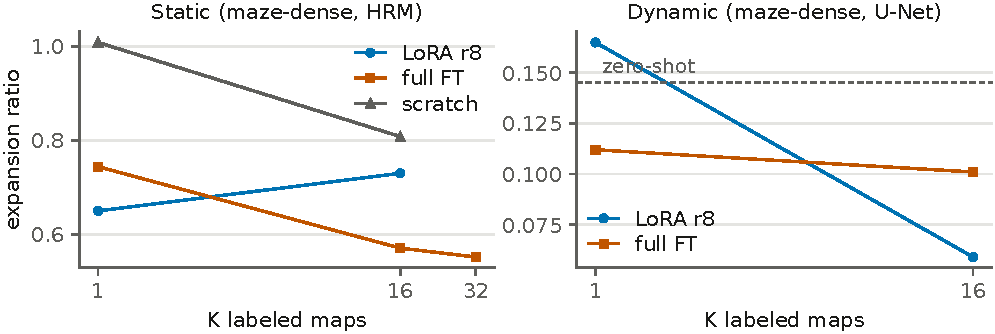
\includegraphics[width=0.98\columnwidth]{figures/fig3_transfer.pdf}
\caption{Illustrative adaptation curves on the static (left) and dynamic (right) dense-maze targets. On this static target, LoRA leads at $K{=}1$ and full fine-tuning overtakes it by $K{=}16$; the sharpest low-label full-fine-tuning failure occurs on the large-rooms target (ratio 1.293 at $K{=}1$; direct contrasts in the text and appendix). On the dynamic target the low-supervision failure is not observed in this $K$-indexed protocol; the matched-label factorial in the text separates the roles of label count and world diversity. Curves connect the evaluated $K$ values for one backbone per panel and are illustrative; quoted inference is map-clustered.}
\label{fig:transfer}
\end{figure}

\textbf{Scarce static labels.} At $K{=}1$, the direct map-paired contrast favors LoRA in all six target/backbone cells: the full-FT$-$LoRA success difference is negative in every cell and significantly so in four (large rooms/HRM $-0.600$ $[-0.773,-0.407]$; bugtrap/HRM $-0.467$ $[-0.587,-0.340]$; large rooms/ON-LSTM $-0.293$; dense maze/HRM $-0.240$; map-clustered intervals). In absolute terms, LoRA retains the zero-shot gain (dense maze ratio 0.686 $[0.590,0.774]$, success $+0.467$), full fine-tuning on large rooms reaches ratio 1.293, and training from scratch on dense maze is significantly harmful (success $-0.167$; Figure~\ref{fig:transfer}). At $K{=}1$, LoRA retains the zero-shot gain, whereas full fine-tuning and scratch degrade it in most cells.

\textbf{Full fine-tuning improves at larger $K$.} At $K{=}16$ the direct contrast reverses on effort: the paired full-FT$-$LoRA expansion-ratio difference is negative (full fine-tuning better) in all six cells and significantly so in five (up to $-0.366$ $[-0.489,-0.235]$ on large rooms/HRM), while the paired success differences are near zero (one cell significantly favors full fine-tuning). The marginal intervals agree (dense maze $K{=}16$: 0.610 $[0.549,0.670]$ versus 0.786 $[0.694,0.891]$, disjoint). A matched-compute ablation compares bounded and unbounded LoRA across 27 cells: the map-level ratio differences have median 0.0000 (standard deviation 0.0077; maximum 0.037), so the near-identical curves suggest the output clamp is not the primary cause of the LoRA plateau. LoRA is not universally protective either: on bugtrap it degrades significantly by $K{=}32$ (ratio 1.153 $[1.012,1.523]$). Full per-cell contrasts are tabulated in the appendix.

\textbf{Dynamic maps supply many labels per map.} The dynamic training run collects 1{,}129{,}536 supervised $(v,t)$ samples from 53 worlds---21{,}312 labeled states per world on average (collection arithmetic in the appendix). At dynamic $K{=}1$, full fine-tuning is not systematically catastrophic and LoRA continues to improve rather than merely preserve the base (Figure~\ref{fig:transfer}, right). Scratch models can post attractive solved-only ratios while solving fewer maps, so success leads those comparisons.

\textbf{A matched-label factorial separates label count from world diversity.} The $K$-indexed protocol confounds two quantities: adding maps adds labels and worlds together. A preregistered factorial therefore holds the number of supervised states $N$ fixed ($N \in \{256, \ldots, 65{,}536\}$) and varies only whether those states are drawn from the fewest worlds that can supply them (\emph{concentrated}) or from eight times as many (\emph{distributed}), in both domains, under matched optimizer steps (protocol, tables, and regression in the appendix). Raw state count does not govern the failure. Concentrated supervision collapses full fine-tuning and scratch in both domains---success $-0.300$ versus the trained source in every seed at dynamic concentrated $N \leq 1{,}024$, and the collapse persists even with $N{=}16{,}384$ states drawn from a single world---while distributing the \emph{same} number of states across more worlds rescues them ($+0.15$ to $+0.20$), with recovery occurring exactly where reaching $N$ forces the sampler onto multiple worlds. Low-rank adaptation collapses in none of the 60 cells. On matched expansion ratios, full fine-tuning is at or below LoRA at every tested $N$ and its interaction with $\log N$ is null, so the protection low-rank adaptation provides at low supervision appears in \emph{success} and is governed by target-world diversity rather than label count. (Dynamic matched-effort cells contain one jointly solved map and support no effort inference; the factorial's conclusions rest on the paired success deltas.)

\section{Scope and Boundary Results}

\textbf{Discrete transfer.} In the complete pooled-multitask grid run, the pooled HRM base improves mean success from 0.591 to 0.612 with lower mean expansions (descriptive); task-specific adapters do not improve broadly. A 3--8-seed pilot on selected 128- and 192-cell maps finds 6--15\% expansion reductions at $w{=}1.0$ with equal or higher observed success; a full-suite confirmation has not been run.

\textbf{Adapter composition did not improve the pooled model.} Interpolating 16 single-family rank-8 adapters by target descriptor routes to the correct family axis (own-axis mass 0.986--0.998), yet map-paired composition never significantly beats the pooled zero-shot model and is significantly worse in two of six cells (ratio deltas up to $+0.098$ $[+0.076,+0.123]$); weight-space and prediction-space mixtures are nearly identical \citep{wortsman2022soups,ilharco2022task}.

\textbf{Architecture and hierarchical depth.} Architecture rankings differ across the tested tasks and input representations: the U-Net is often strongest in the dynamic field study, the HRM holds the lowest single-suite dynamic ratio, and the ON-LSTM leads the early calibrated scalar stage. In compositional multi-leg missions constructed with verified oracle headroom (mission length $K \in \{2,4,8\}$; six learned configurations, three seeds, 54{,}450 evaluation rows), no structured model beats the MLP at two depths with a non-decreasing gap, forced extra recurrent compute yields flat curves, and learned halting moves \emph{opposite} to the depth hypothesis (mean would-halt steps 6.79/7.01/5.30 at $K{=}2/4/8$; map-level $\rho=-0.578$, stratified permutation $p=5\times10^{-5}$). Global-input models do separate from the MLP at shallow missions (ratios ${\approx}$0.67--0.87 in two of three configurations). Five of 33 recurrent cells collapse to constant predictions and are treated as optimization failures rather than capacity estimates. Follow-up experiments on persistent memory, iterative refinement \citep{tamar2016vin,lee2018gppn}, hierarchical substitution, and persistent planning-time state are also negative (persistent carry worsens frontier ranking; MRR delta $-0.0294$ $[-0.0598,-0.0030]$); full gate tables and figures are in the appendix. These are formulation-specific negatives, not claims that recurrence, memory, or hierarchy are universally ineffective \citep{jolicoeur2025trm,czechowski2021subgoal}.

\textbf{Restricted-observation transfer.} A final static study restricts the learned model to a radius-0.20 local subgraph of the roadmap, trained from behavior-derived returns rather than shortest-path labels, and integrates it through one inference-time Bellman backup over that subgraph. Under a preregistered comparison on a disjoint 144-map cohort, this local MLP reduces pooled expansions against the complete-map field HRM by 12.96 (95\% CI $[-16.30,-9.74]$; 109/3/32 wins/ties/losses; every suite mean lower) at better empirical path quality (mean/max cost ratios 1.024/1.162 versus 1.031/1.335), and a separate $w{=}1.10$ bounded control passes all 144 per-instance suboptimality certificates. Sequential ablations attribute the sign change to the backup itself: the same trained model loses by $+16$ expansions under static insertion and wins after one backup. The study is static, uses one model seed and cohort, carries no formal bound on the direct arm, and its prototype feature construction is slower in wall time; full ladder, calibration, and timing tables are in the appendix.

\section{Related Work}

\textbf{Learned guidance for search.} Learned heuristics have been trained by bootstrapping \citep{arfaee2011bootstrap}, oracle imitation \citep{bhardwaj2017sail}, differentiable search \citep{yonetani2021neuralastar}, transformer-based grid guidance \citep{kirilenko2023transpath}, supervised classical-planning objectives \citep{ferber2020neural}, and ranking objectives \citep{chrestien2023rank}. Our work differs in focus rather than mechanism: we retain classical graph search throughout, evaluate cross-family and dynamic transfer of identical trained models, and compare additive against rank-only integration of the \emph{same} predictions \citep{pohl1970,pearl1982semiadmissible,aine2016mha}---a combination these works do not study together.

\textbf{Dynamic, real-time, and motion planning.} The dynamic substrate follows space--time and safe-interval search \citep{silver2005cooperative,phillips2011sipp}. The restricted-observation study is related to real-time heuristic search \citep{korf1990rta} and local value updates in Real-Time Adaptive A\textsuperscript{*} \citep{koenig2006rtaa}; its one-step backup also resembles a single value-iteration-network update \citep{tamar2016vin,lee2018gppn} and neural algorithm execution more broadly \citep{velickovic2021nar}. Unlike those methods, the backup here is applied once, at inference, over a radius-bounded subgraph, purely to integrate a transferred prediction. Learned samplers and end-to-end motion planners \citep{ichter2018sampling,qureshi2019mpnet} replace or augment the planner itself; we retain a fixed classical planner and learn only its guidance, which is what makes heuristic transfer measurable on a PRM \citep{kavraki1996prm}.

\textbf{Adaptation and recursive architectures.} LoRA \citep{hu2021lora}, model soups \citep{wortsman2022soups}, and task arithmetic \citep{ilharco2022task} motivate the low-rank and composition studies; the contribution here is not the use of LoRA but the comparison of low-rank against full-rank updates as a function of planning-label availability. HRM \citep{wang2025hrm}, adaptive computation \citep{graves2016act,banino2021pondernet}, and simplified recursive models \citep{jolicoeur2025trm} motivate the architecture experiments; our results concern heuristic regression and planner integration rather than the benchmark claims of those architectures.

\section{Limitations}

Most continuous primary results are local single-GPU validations with one primary training seed, and several experiments reuse trained bases or test maps rather than constituting independent replications. The dynamic model architecture was selected on the 20-map development cohort, so only the 50-map cohort is selection-free; static budget calibration shares worlds with evaluation (anchor-only, and mitigated by the budget curves, but disclosed); and the baseline set centers on the calibrated anchor plus tuned weighted A\textsuperscript{*}---other strong classical alternatives such as SIPP, and external learned planners, are not compared. The smallest jointly solved cell remains three maps (dense maze), matched-effort magnitudes vary by seed on three of six suites, and a per-suite best-configuration view reported in the appendix is post-hoc. Averaging repeated seeds within maps means quoted intervals underrepresent training-seed uncertainty, which we address only for the dynamic result via across-seed ranges. The discrete rank-only result covers selected cells with 3--8 seeds, not the full 22-suite grid. Map-clustered reanalysis supports the quoted adaptation and architecture conclusions, but not every exploratory table has been regenerated at that grain, and no equivalence tests were run.

The restricted-observation confirmation is static, uses one model seed and one 144-map cohort, and tests whether the transferred signal survives input restriction; it is not evidence about moving obstacles. Its model is locally restricted but the planner still knows the roadmap; this is not map-free sensing. The direct operating point has no formal suboptimality bound, while the certified control is slower, and the prototype feature construction is slower in wall time than complete-map inference despite fewer expansions.

Dynamic obstacles are deterministic, and the work does not cover stochastic prediction, kinodynamic constraints, multi-agent coupling, physical robots, or environments beyond 2-D single-agent navigation. All environments are synthetic; establishing comparability with standardized external benchmarks remains open. Negative results are failures to observe improvement under the pre-specified protocols, not universal rejections of future information, composition, recurrence, memory, or hierarchy. Safety-critical deployment would additionally require uncertainty-aware motion models, collision guarantees, and end-to-end validation.

\section{Conclusion}

Across the tested grid and roadmap domains, learned heuristics generalized to held-out maps and to held-out map families, in both static and dynamic environments. A blind U-Net heuristic selected on a development cohort and frozen before confirmation improved success on all six dynamic test suites---three of them family-level held out---while reducing matched search effort by 73--95\%. The control experiments show that the supervised target and the planner interface can each reverse a model-level conclusion, and the adaptation experiments show a supervision-dependent trade-off: at one labeled map, low-rank adaptation retained the transferred gain where full fine-tuning often degraded it, full fine-tuning became the more search-efficient method as supervision grew, and a matched-label factorial attributes the failure regime to concentration of supervision in too few worlds rather than to label count. Learned planning heuristics should therefore be evaluated jointly with their search interface and supervision budget, not as models in isolation.

\bibliography{references}

% AAAI-27 requires the reproducibility checklist to be uploaded separately
% in the designated submission field; it should not be included in this PDF.

\end{document}
